\documentclass[11pt]{article}
\usepackage{amsmath,amsfonts,amssymb,eucal,graphicx}
\usepackage{epsfig}
%\usepackage{pslatex}
\usepackage{wrapfig}
\usepackage{exscale}
\usepackage{setspace}
\usepackage{subfigure}
\usepackage{color}
\usepackage{url} 
\usepackage{float}
\restylefloat{table}
\usepackage{enumitem}
\usepackage{titlesec}
\titleformat*{\section}{\large\bfseries}
\titleformat*{\subsection}{\normalsize\bfseries}
\titleformat*{\subsubsection}{\large\bfseries}
\titleformat*{\paragraph}{\large\bfseries}
\titleformat*{\subparagraph}{\large\bfseries}
\usepackage[font=footnotesize]{caption}
\usepackage[letterpaper, margin=1in]{geometry}
%\usepackage{showframe}
\usepackage{booktabs}
\usepackage{cite}

\hyphenation{test-bed}

\textwidth  6.6in
\textheight 9.1in
\setlength{\oddsidemargin}{-0.04 in}
\setlength{\topmargin}{-0.7in}
\newcommand{\alex}[1]{\textcolor{cyan}{ #1}}
\newcommand{\noi}{\noindent}
\newcommand{\bi}{\begin{itemize}}
\newcommand{\ei}{\end{itemize}}
\newcommand{\bc}{\begin{center}}
\newcommand{\ec}{\end{center}}

\newcommand{\toc}{{\em IEEE Trans.~Communications, }}
\newcommand{\tit}{{\em IEEE Trans.~Information Theory, }}
\newcommand{\jsac}{{\em IEEE J. Selected Areas Commun., }}
\newcommand{\rtime}[1]{\par\noindent\rlap{#1} \hspace*{2.15cm}}
\newcommand{\iblank}{\par \noindent \hspace*{2.4cm} \hangindent 2.6cm}

\newcommand{\nm}[1]{\textcolor{red}{\textbf{[NM: #1]}}}
\newcommand{\ca}[1]{\textcolor{blue}{\textbf{[CA: #1]}}}
\newcommand{\as}[1]{\textcolor{cyan}{\textbf{[AS: #1]}}}

\def\etal{{\em et al.\/}}
\def\eg{{\em {\em e.g.},\ }}
\def\ie{{\em i.e.,\ }}
\def\etc{{\em etc.\ }}
\def\be{\begin{equation}}
\def\ee{\end{equation}}

\newcommand{\SNR}{{\sf SNR}}
\newcommand{\INR}{{\sf INR}}
\newcommand{\SINR}{{\sf SINR}}
\newcommand{\Nc}{{\cal N}}
\newcommand{\Ec}{{\cal E}}
 
 \newfont{\bb}{msbm10 scaled 1100}
\newcommand{\CC}{\mbox{\bb C}}
\newcommand{\PP}{\mbox{\bb P}}
\newcommand{\RR}{\mbox{\bb R}}
\newcommand{\QQ}{\mbox{\bb Q}}
\newcommand{\ZZ}{\mbox{\bb Z}}
\newcommand{\FF}{\mbox{\bb F}}
\newcommand{\GG}{\mbox{\bb G}}
\newcommand{\EE}{\mbox{\bb E}}
\newcommand{\NN}{\mbox{\bb N}}
\newcommand{\KK}{\mbox{\bb K}}

%\renewcommand{\baselinestretch}{0.965}

\begin{document}

\begin{center}
\textbf{\Large Adaptive Wireless Networks for Spectrally Efficient Communication} \\[0.1in]
\Large DARPA SC2: Functioning Subsystem Design Report \\
Team BAM!\ Wireless
\end{center}

 \section{Introduction}
 In this report, we provide a high-level overview of the functional design for a software-defined radio node employed in a BAM!\ wireless network for the DARPA Spectrum Collaboration Challenge (SC2).  In a BAM! wireless network, a software-defined radio node may operate as either a Standard Radio Node (SRN), or as the Gateway node.  As shown in Figure \ref{fg:BAM-SYS-BD}, the BAM! wireless network includes multiple SRNs and a single Gateway node.  
 \begin{figure} [htb]
 \centerline{
 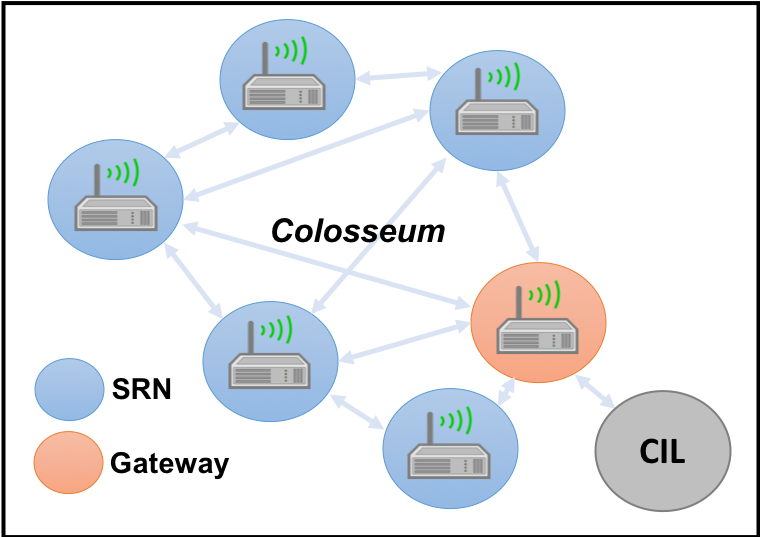
\includegraphics[width = 0.6\textwidth]{Figures/SysBD.png}}
 \caption{BAM!\ Wireless Network for the DARPA SC2.} 
 \label{fg:BAM-SYS-BD}
 \end{figure} 
 Both the SRN and Gateway nodes interact directly with the Colosseum, which orchestrates and emulates specific data transfers and RF scenarios, while only the Gateway node interacts with the Collaborative Intelligent Radio Network Interaction Language (CIL) network. CIL message are defined in accordance with all SC2 competitor networks.  The specific functions provided by each individual BAM! wireless network node (SRN or Gateway) jointly contribute to the realization of a network that functionally adapts to enable simultaneous operation of disparate collaborative wireless networks.  In this report, we highlight the components and key features of each SRN and Gateway node in a BAM! wireless network.
 
 \section{Subsystem Design Components and Features}
 Figure \ref{fg:BAM-SC2-arch} captures the functional components that comprise each BAM! wireless network SRN and Gateway node.  Also shown in Figure \ref{fg:BAM-SC2-arch} - via colored triangles - are the key features for each functional component that ultimately enable collaborative operation at the network level.  Detailed descriptions for each key feature shown in Figure \ref{fg:BAM-SC2-arch} are captured in the list below.
 \begin{figure} [htb]
 \centerline{
 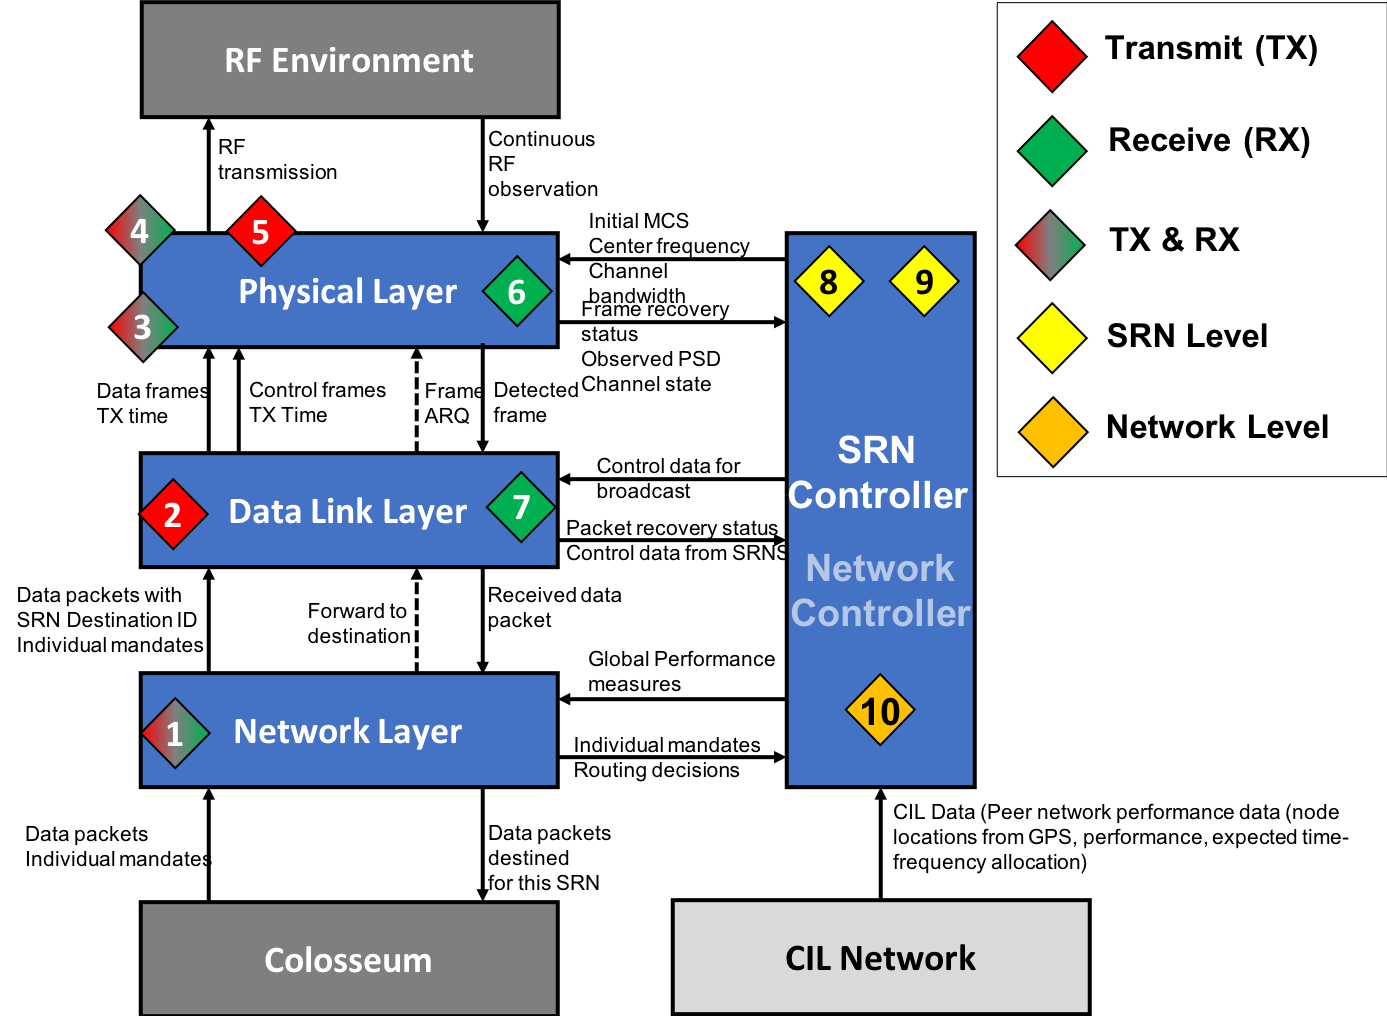
\includegraphics[width = 0.9\textwidth]{Figures/SysFuncBD.png}}
 \caption{Key components and features of a BAM!\ Wireless SRN/Gateway node for the DARPA SC2.   Note that the \emph{Network Controller} component and feature number 10 pertain only to the Gateway node; all other components and features highlighted in Figure \ref{fg:BAM-SC2-arch} are common to all SRN and nodes as well as the Gateway.}
 \label{fg:BAM-SC2-arch}
 \end{figure} 
 
 \begin{enumerate}
     \item \textbf{Multi-hop Routing:} Due to Colosseum emulation of both radio node motion and environment-based physical obstacles (e.g., buildings or terrain), the RF propagation attenuation between any pair of network nodes changes throughout the execution of a scenario.  As such, an information exchange between all unique node pairs may not be possible over the duration of a scenario.  When the scenario specifies an information flow between two network nodes and the link between the two nodes experiences a blockage at some point during the transfer (i.e., information cannot be exchanged between the two nodes), the data traffic associated with the flow can be \emph{routed} through other nodes in the network with links that are not blocked.  In our design, an inter-node blockage is declared by a node when control data cannot be successfully received from another node in the network via the robust control link for a pre-specified amount of time (e.g., 10 seconds).  Alternatively, a link is assumed to be \emph{not blocked} when information sent via the robust control link can be successfully decoded. Using this method, a binary vector can be constructed at every node indicating the link status between itself and all other nodes.  Sharing this information over the robust control channel allows each of the nodes to construct a routing table that is updated periodically throughout the execution of a scenario. Finally, when transmitting data, Dijkstra's algorithm is applied to the current routing table, in order to find the shortest path to the flow destination.
     
     \item \textbf{Transmit Scheduling:} 
     Given the constrained transmit resources at each node and the large number of flows with varying demands, an adaptive scheduling algorithm allocates \textit{time quanta}, and follows a round-robin scheduling scheme.  Time quanta are chosen to maximize both the number of scheduled flows and the efficiency of transmit frames. A flow is only scheduled (i.e., given a non-zero time quantum) if it will likely achieve its performance thresholds with its assigned quantum.   A variant of round-robin scheduling, termed deficit round-robin flow queue scheduling (illustrated in Figure \ref{fg:DeficitRR}) gives better fidelity to the assigned time quanta and enables customized functionality (e.g., ARQ) for each flow's queuing scheme.
     \begin{figure} [htb]
     \centerline{
     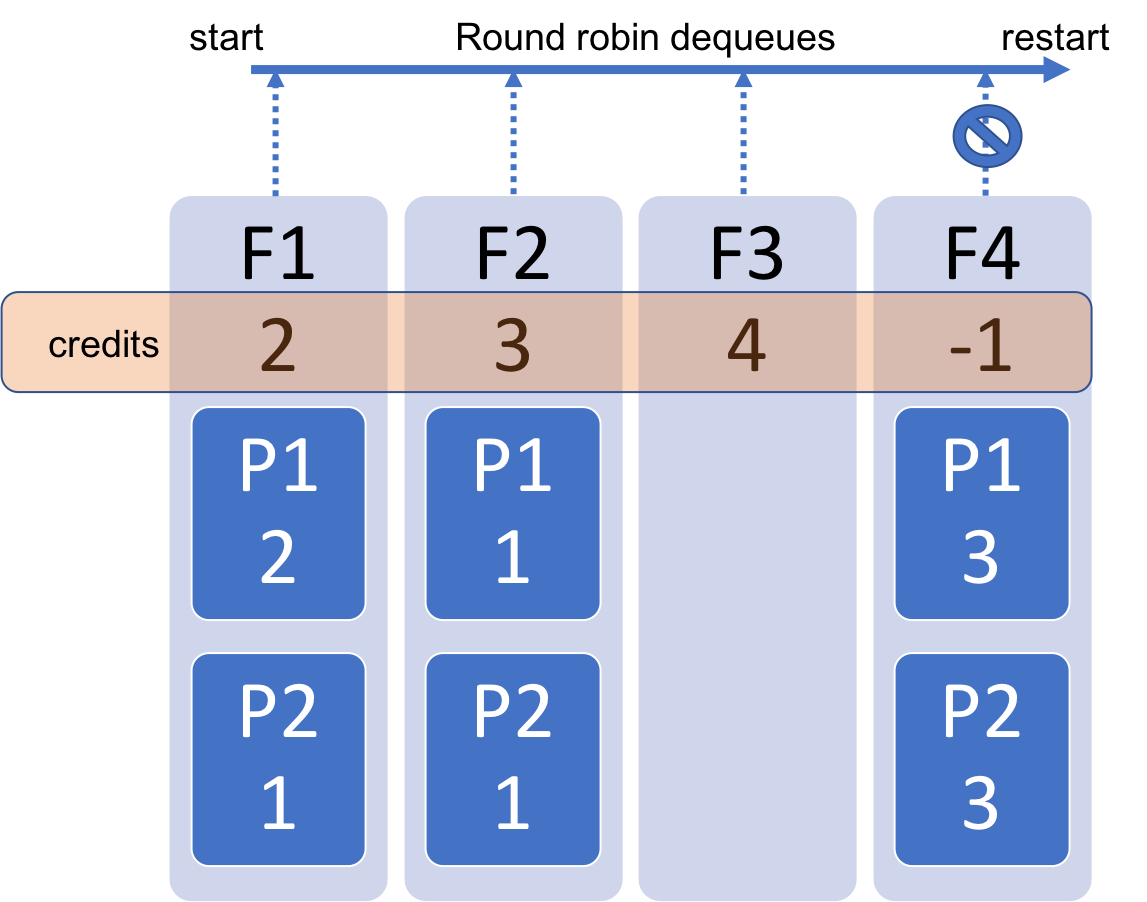
\includegraphics[width = 0.6\textwidth]{Figures/DeficitRR.png}}
     \caption{Example of deficit round-robin flow queue scheduling where flow queues $F\#$ with credits ($\#$) containing packets $P\#$ of size ($\#$) are scheduled.}
     \label{fg:DeficitRR}
     \end{figure}
     
     \item \textbf{Broadcast of Control Data:}
     The protocol followed to transfer network control data consists of two different message structures, where each message structure is transmitted with a different modulation technique. 

     The first type of control message, which we will refer to as the \emph{short} control message, is transmitted using a non-coherent 8-FSK modulated link with 480 kHz of bandwidth, Reed-Solomon error control coding, and a robust time-hopping synchronization scheme, as shown in Figure \ref{fg:NDASync}.
     \begin{figure} [htb]
     \centerline{
     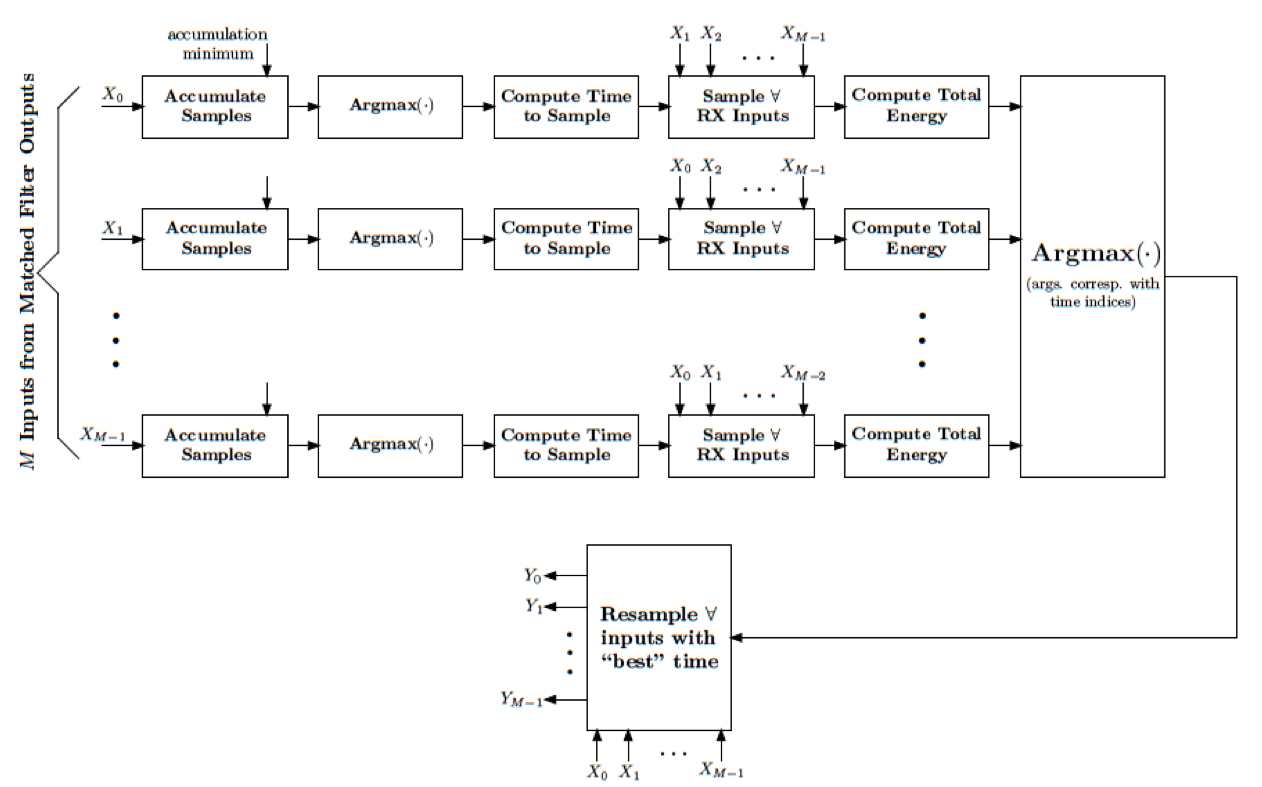
\includegraphics[width = 0.9\textwidth]{Figures/NDASync.png}}
     \caption{Robust synchronization method developed for the low signal-to-interference ratio scenario of the DARPA Spectrum Challenge leveraged for the BAM! wireless robust control link.}
     \label{fg:NDASync}
     \end{figure}
     The center frequency of this control channel changes every second between the upper and lower band edge, that are determined by the Colosseum environment.
     
     The medium access method of the FSK control channel can best be described as a variant of slotted ALOHA without the collision detection and backoff mechanism. At every slot boundary (the slot period is set to 60 ms), each SRN transmits a short control packet with probability $1/N$, where $N$ is the number of nodes in the network. Collisions result in decoding errors and are discarded at the receiver. Information in this short control message includes the number of SRNs in the network, the current channel allocation, and a timestamp. When a SRN receives updated information, it re-broadcasts this modified state. This approach results in a robust broadcast topology that is used for network bootstrapping, initial node discovery, and as a fallback control link in high-interference environments.

     The second type of control message is transmitted using the DFT-s-OFDM high rate data link, and includes additional information such as traffic statistics and feedback on the performance of individual mandates. Since a center frequency is assigned to one SRN at a time, these messages are transmitted using the center frequencies assigned to each node in a broadcast fashion. These \emph{long} control messages are broadcast every second interleaved with the data traffic.
     
     Figure \ref{fg:CCEx} shows the power spectrum observed by a single SRN during a qualification scenario run on the Colosseum.  Note that the narrowband transmissions at the upper and lower band edges are short control messages; the four wideband channels contain both long control messages and data.
     \begin{figure} [htb]
     \centerline{
     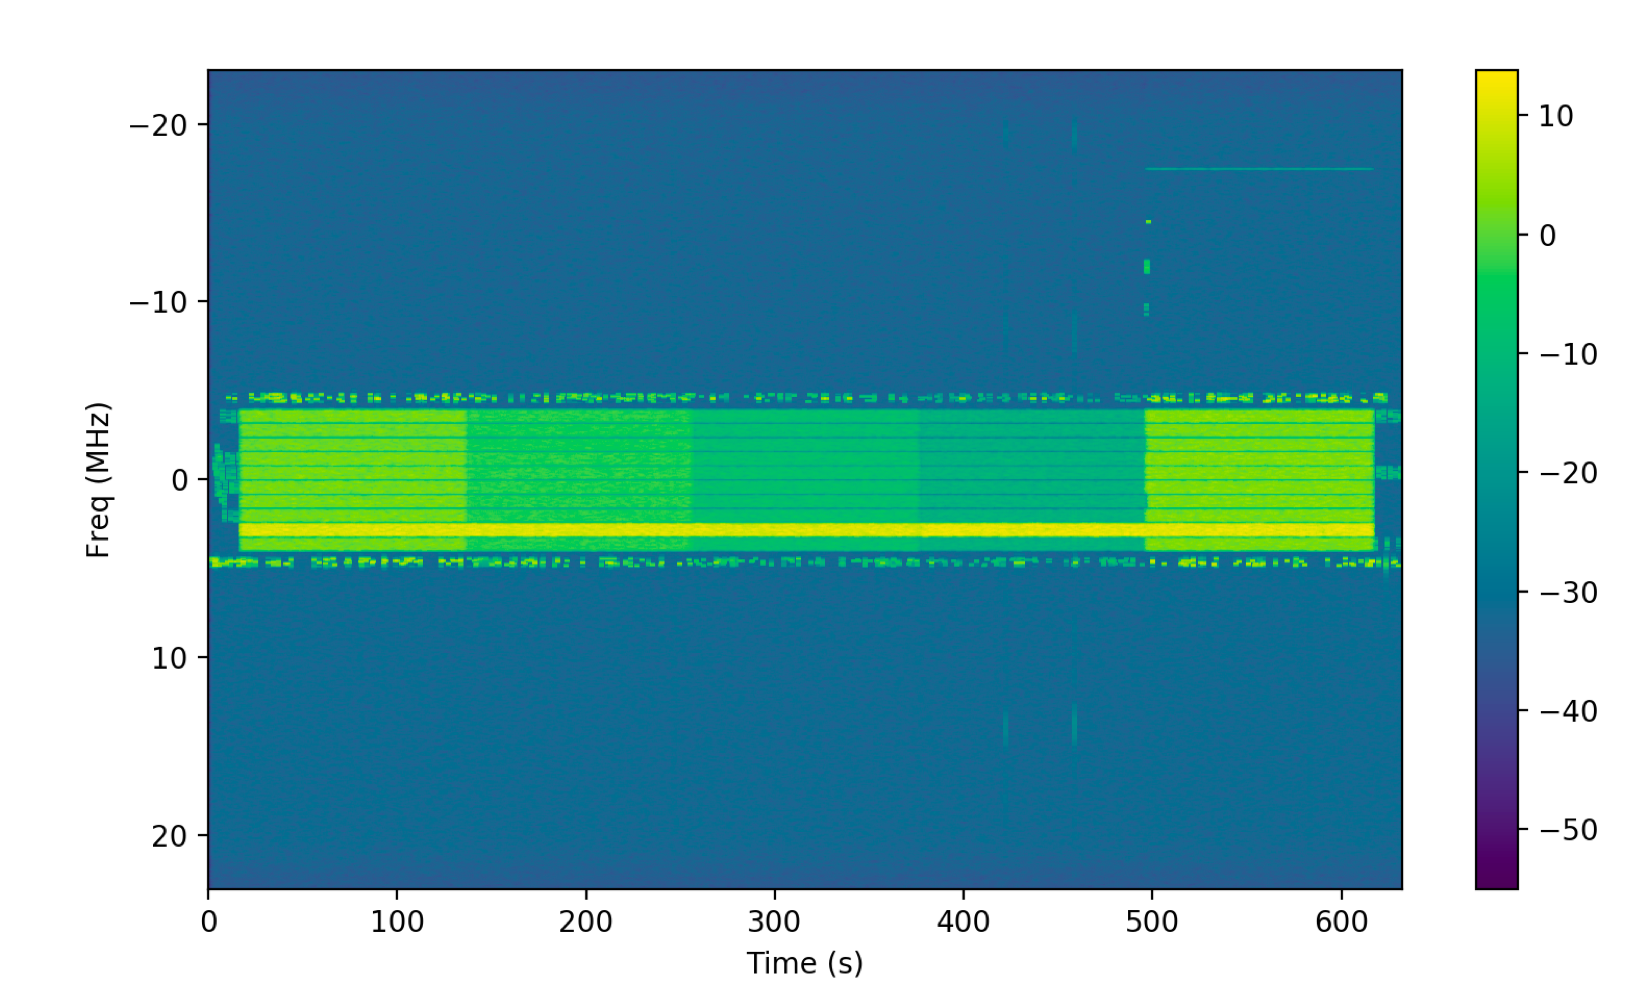
\includegraphics[width = 0.6\textwidth]{Figures/CCEx.png}}
     \caption{Control transmissions observed in SRN power spectrum.}
     \label{fg:CCEx}
     \end{figure}

     \item \textbf{High Rate Data Link:}
     Both mandated and un-mandated traffic is transmitted using a DFT-spread Orthogonal Frequency Division Multiplexing (DFT-s-OFDM) waveform of varying bandwidth and center frequency and power spectrum as shown in Figure \ref{fg:PowSpec}. Each SRN in the network is assigned to a specific center frequency and bandwidth (sometimes referred to as \emph{channel}) at any point in time as determined by the channel allocation algorithm (see feature $\#$10 for more information). Every SRN tunes its $N-1$ receive chains to these $N-1$ channels, where $N$ refers to the number of SRNs in the network, and is able to receive transmissions from all other SRNs in the network. Independent of the bandwidth assigned to a node, all waveforms occupy 128 subcarriers of which 108 are used for data symbols, 12 are used for pilot symbols, and 8 subcarriers are null transmissions used for noise variance estimation required for optimal reception and adaptation of modulation and coding state.  
     \begin{figure} [htb]
     \centerline{
     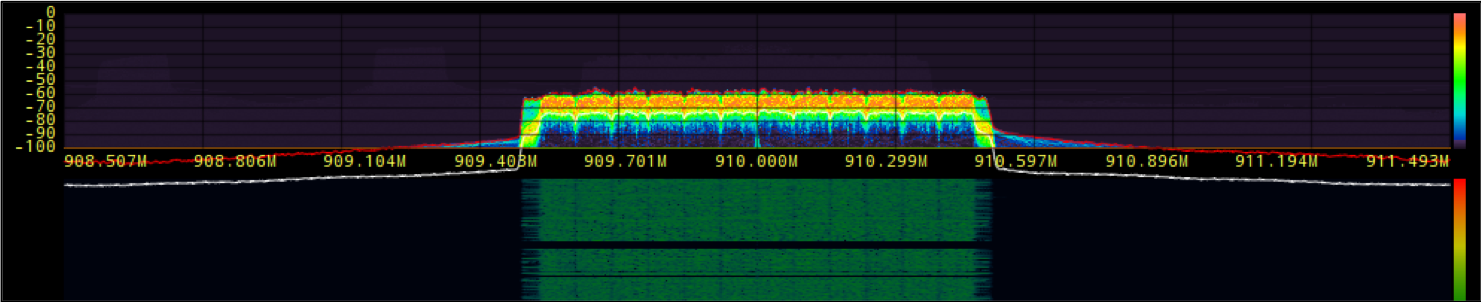
\includegraphics[width = 0.8\textwidth]{Figures/PowSpec.png}}
     \caption{The power spectrum of the DFT-s-OFDM waveform.}
     \label{fg:PowSpec}
     \end{figure}
     The receivers perform Schmidl \& Cox time synchronization and frequency offset compensation. Channel and noise variance estimation is performed in the frequency domain, followed by frequency-domain equalization. Payload data is modulated using either QPSK, $16$-QAM, $32$-QAM or $64$-QAM rectangular constellations. The channel code is the IEEE 802.11 QC-LDPC suite of codes, consisting of parity check matrices for rates $1/2$, $2/3$, $3/4$, and $5/6$.  Block error rate curves for the different combinations of code rates and modulation constellations are shown in Figure \ref{fg:BLER}.
     \begin{figure} [htb]
     \centerline{
     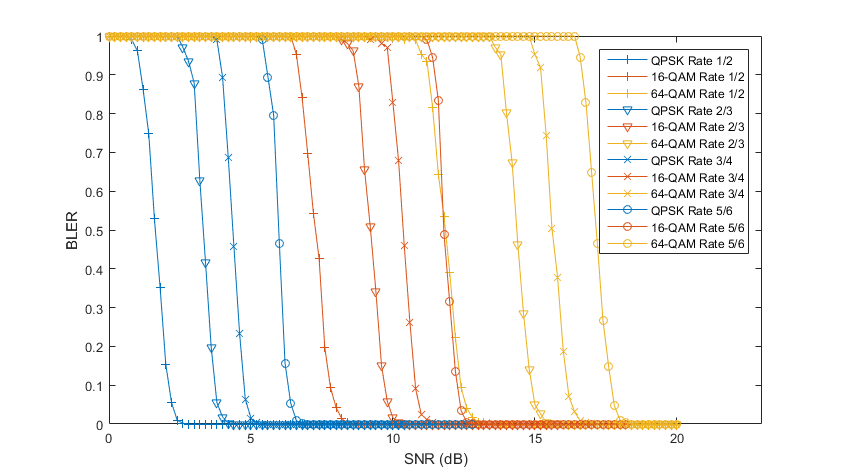
\includegraphics[width = 0.6\textwidth]{Figures/BLER.png}}
     \caption{Simulated block error rate curves (BLER) for all combinations of modulation order
     and code rate supported by a BAM! wireless SRN.}
     \label{fg:BLER}
     \end{figure}

     The fundamental unit of transmission on the physical layer is a Frame, which is comprised of a Frame header and a payload. Frame headers are always modulated using QPSK and coded using the rate $1/2$ LDPC code. Information in the frame header consists of the source and destination SRN ID, the MCS index (indicating modulation and coding scheme) chosen for the payload, and the number of blocks (codewords) contained in the payload. Frame headers are furthermore protected using a $32$-bit cyclic redundancy code and contain a unique identifier (frameID) for logging purposes.

     Frame payloads consist of a sequence of blocks (codewords of the chosen channel code) modulated according to one of the available modulation schemes and mapped to subcarriers of a sequence of OFDM symbols. The information bits of the sequence of payload blocks is obtained from a sequence of \emph{segments}, which are Layer 2 units of data. A segment can be one of the following types: IPv4 segment carrying Colosseum Data, IPv4 Segment with ARQ information, or control segment.
     
     

     \item \textbf{Transmit Power Control:} 
     In our design, transmit power control is employed on a per-node basis for the protection of passive incumbents. Transmit power control is not currently used for any other scenarios.  For scenarios that include passive incumbents, each incumbent periodically broadcasts (to all networks) its current center frequency, bandwidth, current measurement of the total receive power, and a receiver power threshold via the CIL network.  Note that the bandwidth, center frequency, and threshold may change throughout the scenario.  When the power measured by an incumbent exceeds its current power threshold setting, the networks participating in the scenario are required to collectively lower their per-node transmit powers so that total power at the passive incumbent drops below the threshold. Similarly, when the power measured by the incumbent is below the threshold, the network nodes may (but not required to) increase transmit power as long as the total measured power remains below the threshold.  Our approach leverages data from the CIL network to determine the total number of nodes $N$ (over all networks including the BAM! wireless network) currently transmitting in the frequency band observed by the passive incumbent.  Assuming non-coherent power combining at the passive incumbent, the transmit power for each node in the BAM! network currently transmitting over the channel observed by the passive incumbent adjusts its transmit power (if possible) by an amount proportional to the difference between the incumbent's measured power and the threshold divided by $N$. This formulation assumes that power adjustments across the networks are done in a fair way (i.e., all networks make similar power adjustments). 
     
     \item \textbf{Adaptation of Modulation Order and Error Control Coding Rate:}
     Our approach to adaptive and joint selection of the modulation order (i.e., the constellation size) and code rate aims to maximize the raw throughput of a particular link, by finding the combination of modulation order $M$ and code rate $R$ that results in the smallest Euclidean distance between circles centered about adjacent constellation symbols, with radius proportional to the ratio of estimated standard deviation of additive noise plus interference and asymptotic code gain.  This maximization is subject to two different constraints which effectively reduce the size of the feasible set of options:
     \begin{itemize}
         \item The selected $M$ and $R$ must satisfy a lower bound on throughput.
         \item Given an estimate of additive noise variance, the selected $M$ and $R$ must have a predicted block error rate that satisfies a pre-specified upper bound.
     \end{itemize}
     Note that a closed form approximation for block error rate as a function of minimum constellation distance and noise standard deviation is assumed when evaluating the second constraint.  A sliding window median filter is also applied to estimated noise variance in attempt to remove noise variance measurements with low probability of occurrence.  An example of the illustrated adaptive algorithm is shown in Figure \ref{fg:MCS} for a test Payline scenario run on the Colosseum.
     \begin{figure} [htb]
     \centerline{
     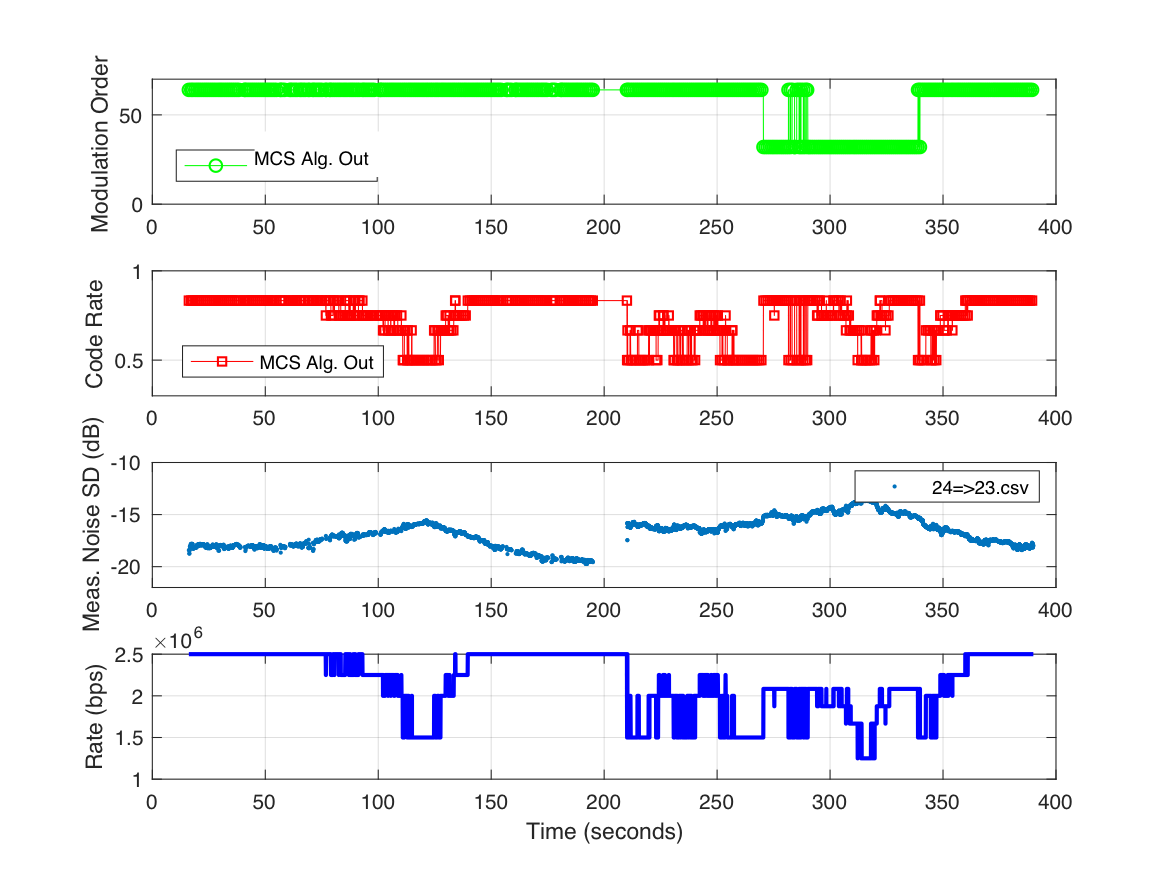
\includegraphics[width = 0.8\textwidth]{Figures/MCS.png}}
     \caption{Adaptation of modulation order and code rate due to change in the standard deviation of additive noise.  It is important to highlight that the link rate reduces as the measured standard deviation of the additive noise increases.}
     \label{fg:MCS}
     \end{figure}
     
     \item \textbf{Automatic Repeat Request (ARQ):}
     Reliable transmissions and an automatic repeat request (ARQ) mechanism are handled by the Data Link and Network layers. Each flow is evaluated for the necessity of reliability and the parameters pertinent to the ARQ algorithm.  When the performance thresholds indicate a file type of flow, ARQ is turned on to ensure the packets of the flow are reliably sent across each leg of the network.  Bursty UDP flows (i.e., simulated file transfers) are specially detected and handled.  Each burst is identified and the packets within a burst are sequenced by the sender.  The receiver provides positive acknowledgements of sequence numbers within a burst.  A special flow queue (see feature \#2 above) then dynamically re-enqueues packets for re-transmission based on the ARQ feedback.  The special flow queue to handle ARQ transparently provides the necessary information to the scheduler.
    
     \item \textbf{Program Configuration:}
     A database of options allows a single version of BAM!\ Radio to be configured for various experiments and scenarios.  The database has harmonious and sensible default values.  Both command line arguments and configuration files may be given to the radio program to customize the database at the time of execution.

     \item \textbf{Calculation and Visualization of Performance Measures:}
     Subsystems of our radio design can emit events which are logged to a structured SQLite database at each SRN. As part of the post-processing step of a Colosseum job, these databases are merged into a final database containing all available information about the job. This database is used as an input into our analysis tools. Our main analysis tool consists of the custom GUI application (shown in Figure \ref{fg:GUI}), which displays a variety \begin{figure} [htb]
     \centerline{
     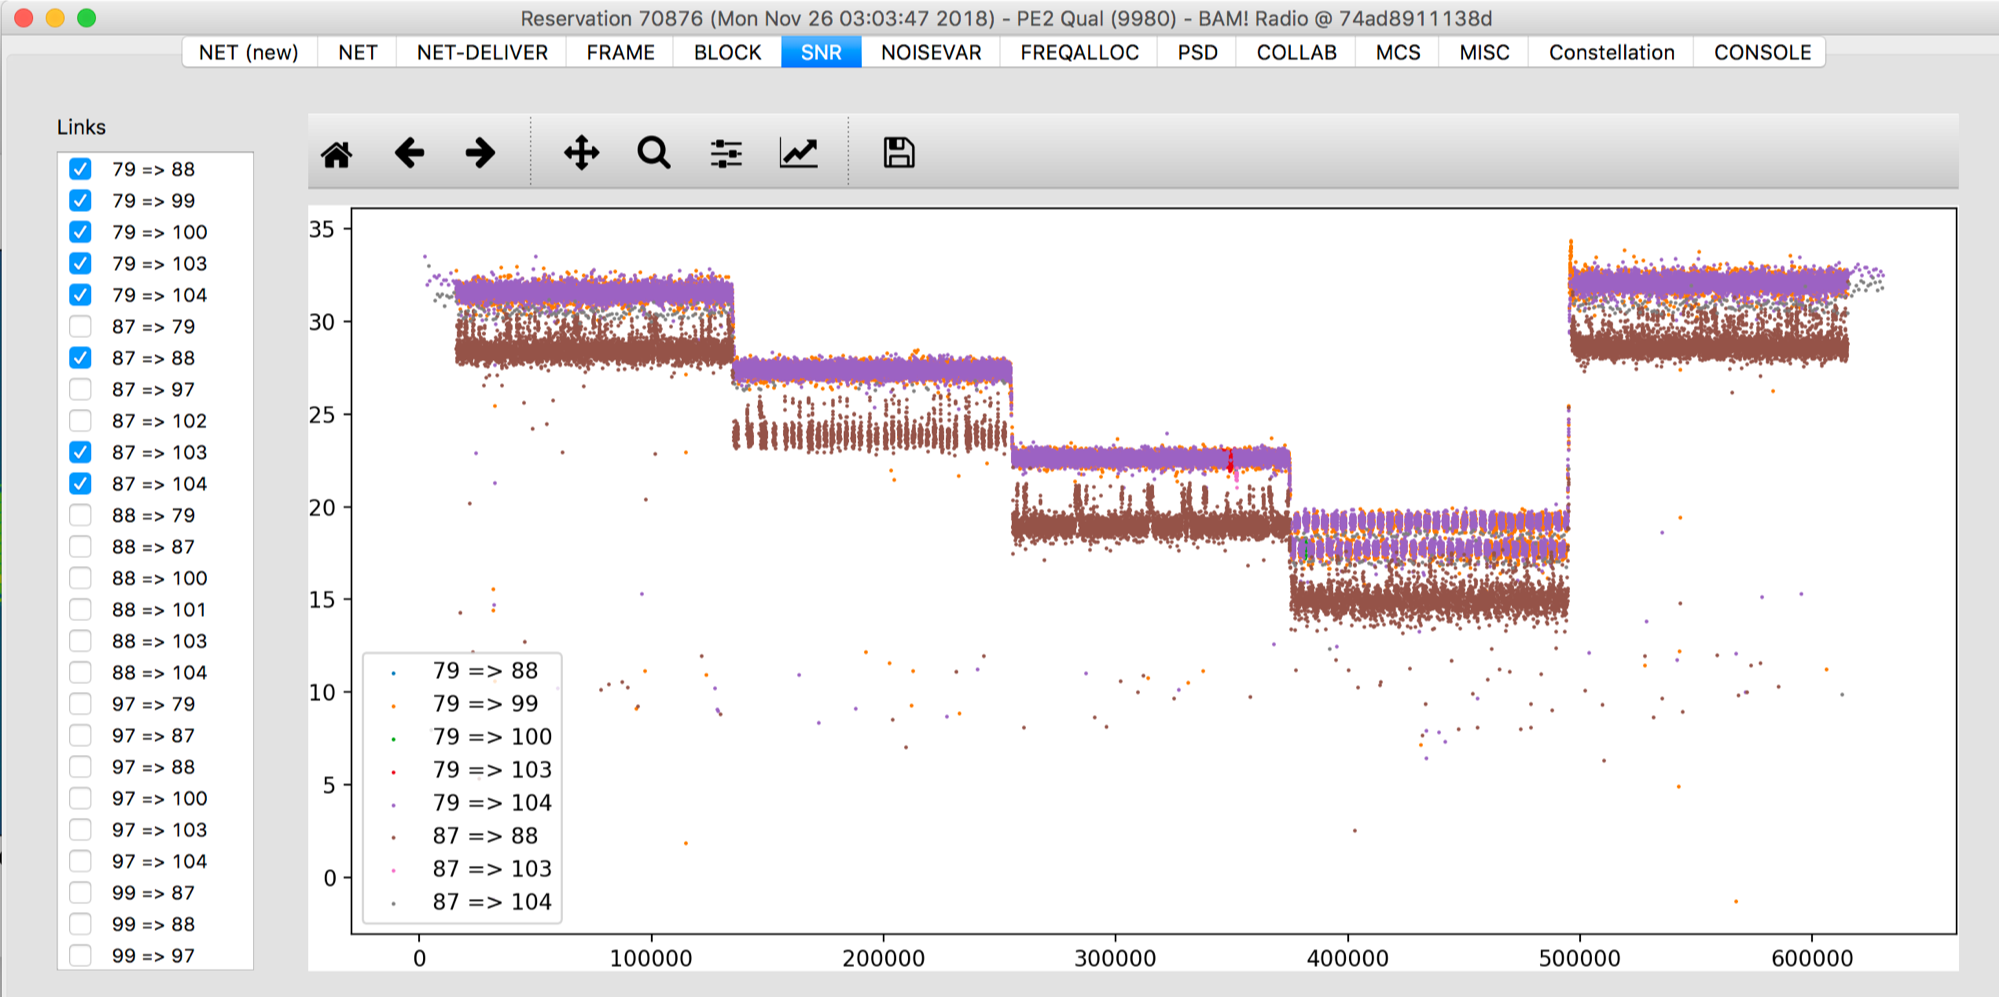
\includegraphics[width = 0.8\textwidth]{Figures/GUI.png}}
     \caption{BAM! wireless SNR measurement tab of the analyzer GUI.}
     \label{fg:GUI}
     \end{figure}
     of metrics from the scenario including the sum data rate offered by the Colosseum, the sum and per-flow delivered data rate, sum and per-flow latency, sum and per-flow reported mandates, per-link frame error rate, per-link block error rate, per-link receive signal-to-noise ratio, per-link additive noise variance, per-link allocated transmit frequency and bandwidth, per-SRN measured power spectral densities, CIL messages transmitted and received by the Gateway, per-link modulation and coding state, and per-link observed signal constellations.
     
     In order to fully assess our network's performance during a particular Colosseum scenario, additional visualization tools have been constructed such as tables that map links and flows (due to multi-hop, a flow may have more than one link associated with it), network connectivity graphs that assist in the debugging of multi-hop routing decisions, and a plot of SRN location over time (see Figure \ref{fg:Loc} for an example) for a particular scenario to help us better understand our measured performance.
     \begin{figure} [htb]
     \centerline{
     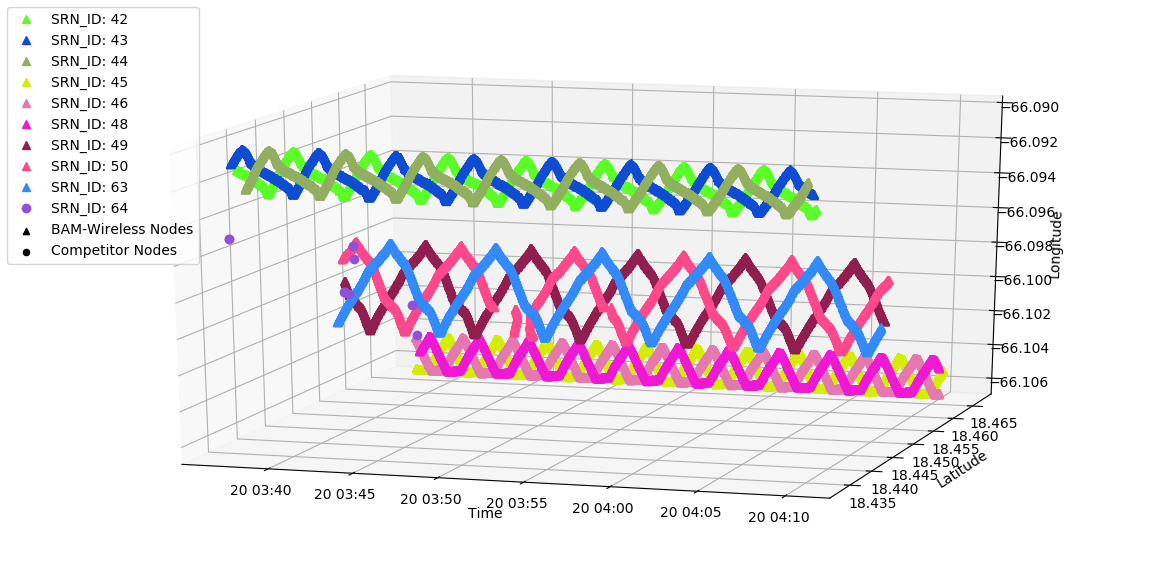
\includegraphics[width = 0.8\textwidth]{Figures/Payline_24Nov2018_LocationPlot.png}}
     \caption{SRN location plot from a Payline test scenario run on Colosseum.}
     \label{fg:Loc}
     \end{figure}
     
     \item \textbf{Channel Allocation Algorithm:}
     There are certain triggering conditions for a reallocation of channels. Specifically, we keep track of both our own and other teams' performances, and if we have been the worst performing team in terms of the number of individual mandates achieved for a certain period, then we reallocate all channels. On the other hand, if we have been achieving at least a certain number (e.g., 2) of mandates above the ensemble minimum, then we reduce the bandwidth of our channels while maintaining their center frequencies in order to free up spectrum resources. The channel reallocation will also be triggered when there is an environmental update or a change in the offered set of individual mandates. When a reallocation is triggered, the bandwidth assigned to each channel is determined based on the amount of available resources, the offered traffic to the corresponding node, and the estimated quality of our links. Figure \ref{fg:ChanAllocEx} shows an example of the spectrum occupied by the BAM! wireless network (as observed by one SRN) during a match setup based on the Alleys of Austin scenario.
     \begin{figure} [htb]
     \centerline{
     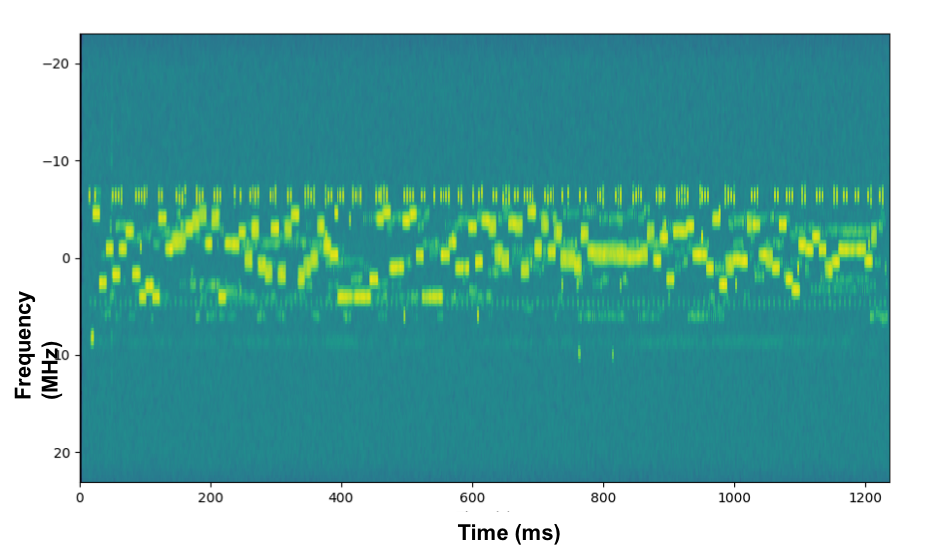
\includegraphics[width = 0.6\textwidth]{Figures/ChanAllocEx.png}}
     \caption{Spectrum occupied by BAM! wireless network as a result of performance-based network level channel allocation.}
     \label{fg:ChanAllocEx}
     \end{figure}

     The channel allocation algorithm aims to find center frequencies that minimize interference from/to other teams based on CIL SpectrumUsage and LocationUpdate messages. Specifically, we first estimate the channel gain between each pair of nodes based on their location and an empirical path loss exponent. We then estimate the amount of interference suffered by each of our nodes at each frequency band, based on the channel gain and the transmit power obtained from SpectrumUsage messages. We then use a heuristic search to determine the center frequencies that minimize the total amount of interference at our receiving nodes.
 \end{enumerate}
 
 \section{Future Work}
 The following list summarizes planned future work and enhancements for the BAM! wireless network.
 \begin{itemize}
     \item Generation and use of non-binary routing tables as part of the multi-hop routing feature.
     \item Late effort during Phase 2 involved a complete redesign of the data gathering and decision making mechanisms at the gateway node. Future work involves adapting our current decision making algorithms to use this more structured approach and to access the additional data that is now being recorded. 
     \item Incorporation of transmit power level into the adaptive modulation and coding state algorithm.
     \item Noise whitening to improve link performance in the presence of narrowband interference.
     \item Use of multiple antennas for transmit beamforming to maximize the receive SNR.
     \item Incorporation of an intelligent scenario identification algorithm, that will be trained and tested using Colosseum Free Play matches.
     \item Enabling conversations through CIL to negotiate spectrum allocation with peer networks, with the goal of maximizing the ensemble performance.
     
 \end{itemize}
 
 \section{Conclusion}
 In this report, we presented the functional design for nodes within the BAM! wireless radio network. Our design is compatible with Colosseum CIL messages, and incorporates them to effectively contribute to an orchestrated ensemble intelligence for the SC2 Challenge. The functional components of our current system, and their interconnections, were depicted in Figure~\ref{fg:BAM-SC2-arch}. Design details for each component were then given, as well as validation results obtained from testing on Colosseum. Our plan for future work in Phase 3 was finally provided. 
\end{document}
